\documentclass{beamer}


\usepackage{siunitx}
%for boxes
\usepackage{tcolorbox}
\usepackage{amsmath}
\usetheme{UoB}
\addtobeamertemplate{navigation symbols}{}{%
    \usebeamerfont{footline}%
    \usebeamercolor[fg]{footline}%
    \hspace{1em}%
    \insertframenumber/\inserttotalframenumber
}


\newcommand{\vc}[1]{\vec{\boldsymbol{#1}}}
\newcommand{\hi}{\hat{\boldsymbol{i}}}
\newcommand{\hj}{\hat{\boldsymbol{\text{j}}}}
\newcommand{\hk}{\hat{\boldsymbol{\text{k}}}}
\usepackage{mathtools}
\newcommand\deq{\stackrel{\mathclap{\tiny\mbox{def}}}{=}}
\usepackage{soul}

%block size
\setbeamerfont{block title}{size=\small}

\makeatletter
\let\HL\hl
\renewcommand\hl{%
  \let\set@color\beamerorig@set@color
  \let\reset@color\beamerorig@reset@color
  \HL}
\makeatother

\usefonttheme{serif}
%\usefonttheme{professionalfonts}
 \usepackage{eulerpx} % Euler math font
\usepackage{color} \definecolor{lightblue}{rgb}{.90,.95,1} 
\sethlcolor{lightblue}

\usepackage{animate}
\title[Short Title]{Potentials and Fields}
\subtitle{in the context of electromagnetism}
\author{Francesco Turci}
\institute{School of Physics}
\date{7th February 2023}


%solve eulerpx bug
\DeclareMathSymbol{\infty}{\mathord}{symbols}{49}
\begin{document}
\lecture{Lecture 1}{01}


\begin{frame}[leftcolor=white,rightcolor=UniversityRed,div=0.8\paperwidth]
  \titlepage
\end{frame}



\begin{frame}
\frametitle{Repository \& references}
All the resources can be found on the dedicated repository:
\href{}{}


Additional context and information can be found in
\begin{itemize}
	\item Chapter 23, \textit{Physics for Scientists and Engineers}, Tipler and Mosca
\end{itemize}
	
\end{frame}

\begin{frame}
	\frametitle{Goals}
	\begin{itemize}
		\item Recall the ideas behind conservative forces and potential energy.
		\item Introduce the concept of potential in electrostatics.
		\item Contrast the electric and magnetic cases. 
	\end{itemize}
\end{frame}

\begin{frame}

\frametitle{Conservative forces}
\small

Under the action of conservative forces, the \textbf{mechanical energy is conserved}.
\begin{equation}
E^{i} = K^{i}+U^i = K^{f}+U^f= E^f.
\end{equation}
Hence
\begin{equation}
	\Delta U = U_f-U_i = - (K_f-K_i)
\end{equation}

\pause
\textbf{Work} can be introduced via the kinetic energy theorem
\begin{equation}
	W  =K_f-K_i,
\end{equation}
so that (using the scalar product notation for W)
\begin{equation}
	\Delta U = U_f-U_i = - W   = -\int_i^f \vc{F}\cdot d\vc{\ell}
\end{equation}
\pause
\hl{The work done by a conservative force only depends on the \textbf{initial} and \textbf{final} positions.} It is a function of the spatial \textbf{configuration}.
	
\end{frame}

\begin{frame}
	\frametitle{Potential energy and path independence}
\small


	\begin{block}{\textbf{Potential Energy Difference}}
\begin{equation}
	\Delta U=U_f-U_i=-\int_{i}^{f} \vc{F} \cdot d \vc{\ell}
	\label{eq:udef}
\end{equation}
\end{block}
\begin{center}
	
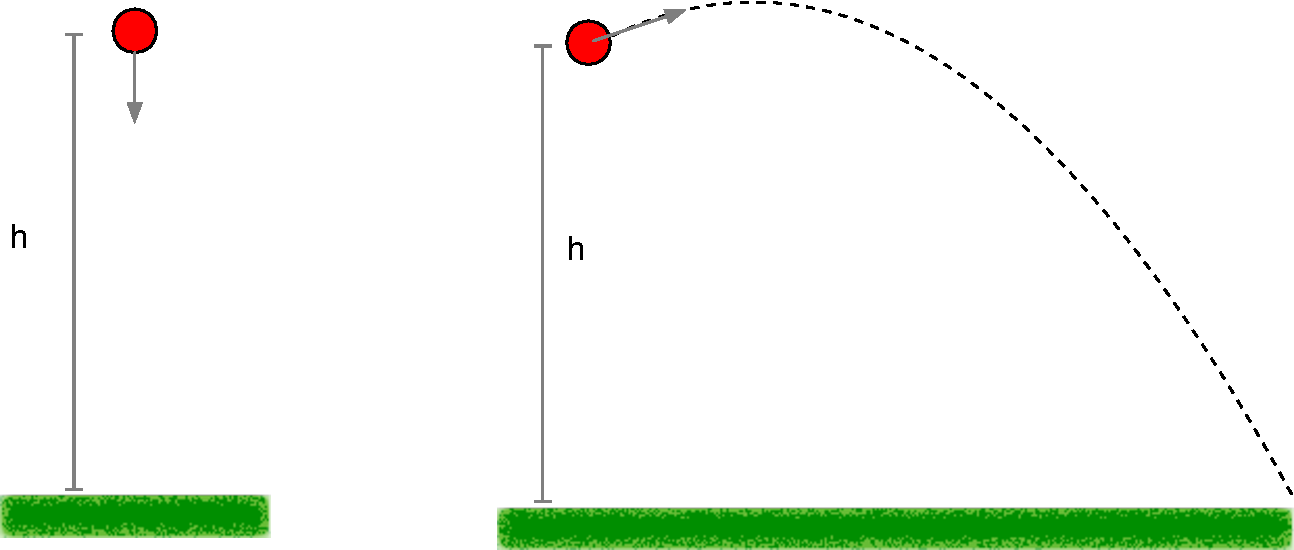
\includegraphics[width=0.8\columnwidth]{figs/paths}
\end{center}
	
\hl{Same initial and final positions, same potential energy difference.}
\end{frame}

\begin{frame}
\frametitle{Potential energy and path independence}
\small

For a closed path $C$, the initial position is also the final position, hence
\begin{block}{Circulation}
	\begin{equation}
	\mathcal{C} = \oint_C  \vc{F} \cdot d \vc{\ell} = 0
\end{equation}
\end{block}
For \textbf{any} closed path, the circulation of a conservative force is \textbf{zero}.\newline
\pause

Conservative forces include:
\begin{itemize}
	\item the gravitational force
	\item the elastic force
	\item the electrostatic force
\end{itemize}

	
\textbf{Q:} Can you think of some \textbf{counter-examples}?
\end{frame}


\begin{frame}

\frametitle{Electric potential difference}
\small 
We can define the electrostatic field from the electrostatic force  using the test charge $q$:
\begin{equation}
	\vc{E}= \dfrac{\vc{F}_e}{q}
\end{equation}
For an infinitesimal displacement, the definition of $\Delta U$ (eq.\ref{eq:udef}) implies

\begin{equation}
	dU = - \vc{F}_e\cdot d\vc{\ell}= -q\vc{E}\cdot d\vc{\ell}.
\end{equation}
This suggests defining a new quantity
\begin{block}{Potential Difference}
\begin{equation}
	dV = -\vc{E}\cdot d\vc{\ell}.
\end{equation}
\end{block}
and naturally $dU = q dV$.

\end{frame}




\begin{frame}
\frametitle{Electric potential}
\small

Let us consider $dV = -\vc{E}\cdot d\vc{\ell}$ and different possible displacments $d\vc{\ell}$.

\begin{itemize}
	\item If $d\vc{\ell}\perp\vc{E}\rightarrow dV=0$.
	\item If $d\vc{\ell}\parallel \vc{E}\rightarrow dV=dV_{\text{max}}$
\end{itemize}
The projection of $\vc{E}$ along the displacement is 

\begin{equation} \vc{E}\cdot d\vc{\ell}= E cos\theta d\ell \deq E_t d\ell \rightarrow E_t = -\dfrac{dV}{d\ell}
\end{equation}

Suppose we know $dV$ and want to retrieve $\vc{E}$. We now know that
\begin{itemize}
	\item we need to move by $d\vc{\ell}$ in the direction of greatest change in $V$
	\item the magnitude of $\vc{E}$ in that direction is the derivative along $d\vc{\ell}$
\end{itemize}
These are the defining properties of the \textbf{gradient} of $V$.



\end{frame}%The notation $dV$ indicates that there exists a differentiable function $V$ that we call \textbf{potential} that depends only on the configuration of the charges.

\begin{frame}
\frametitle{Electric potential}
\small

%
%The potential difference 
%
%\begin{equation}\Delta V = \int_i^f dV = V_f-V_i =-\int_i^{f}\vc{E}\cdot d\vc{\ell}\end{equation}. 
%
%This signifies that the integral over the path connecting $i$ and $f$ only on the
%
% we link the vector field $\vc{E}$ to the potential 

\begin{block}{Field as gradient of potential}
\begin{equation}
		-{\rm grad} V(\vc{r}) = -\vc{\nabla}V(\vc{r}) = \vc{E}(\vc{r})
\end{equation}
\end{block}
Naturally \begin{equation}\Delta V = V(\vc{r})-V(\vc{r}_0) =\int_{\gamma(\vc{r}_0, \vc{r})} \vc{\nabla}V(\vc{r})d\vc{r}=-\int_{\gamma(\vc{r}_0, \vc{r})} \vc{E}(\vc{r})d\vc{r},
\end{equation}
on any path $\gamma$ between $\vc{r}_0$ and $\vc{r}$.


\begin{itemize}
%	\item $V(\vc{r})$ can be evaluated along any path, and takes value for any point in space $\vc{r}$.
	\item $V(\vc{r})$ is a \textbf{scalar} function , $\mathbb{R}^3\rightarrow\mathbb{R}$
	\item Only $\Delta V$ are physically significant, i.e. one must define a reference configuration $\vc{r}_0$ with zero potential $V=0$. 
	\item The potential is measured in \textbf{Volt}, $\unit{1\volt}= 1\unit{\joule}/1\unit{\coulomb}$
\end{itemize}

\end{frame}





\begin{frame}
\frametitle{Example 1: single point charge}
%Take a positive point unit charge $Q_1 = +1\unit{\coulomb}$  at $P_1 = (0,0)\unit{\meter}$. 
\small
The electric field at a distance $r$ from a charge $q$ 

$$\vc{E}=\frac{k q}{r^2} \hat{\boldsymbol{r}}$$
Taking the integral definition of $V$ and a reference point at $r_{0}=+\infty$ with $V(\infty)=0$ we have
$$V(\vc{r})-V_{\infty }=-\int_{\infty }^{\vc{r}} 
\vc{E} \cdot d \vc{\ell}=-\int_{\infty }^{\vc{r}}
\frac{k q}{r'^2} \hat{r'} \cdot d \vc{\ell}=-
\int_{\infty }^{r} \frac{k q}{r'^2} d r'
$$
\begin{block}{Coulomb potential}
	\begin{equation}
		V(r) = \dfrac{kq}{r} \quad \text{(central potential)}
	\end{equation}
\end{block}

The work required to move a test particle $q_0$ at rest at $r=\infty$ to distance $r$ from $q$ is {$W=kq q_0/r$}.


\end{frame}

\begin{frame}
	\frametitle{Example 2: equipotential lines and field lines}
	
	For a system composed of multiple charges, the superposition principle holds for the potential as well:
	\begin{equation}
		V_{\rm total} =\sum_{k=1}^N V_k
	\end{equation}
	The potential is a scalar function that complements the picture provided by the field lines:\newline
	{\color{UniversityRed}\href{https://electric-charges.herokuapp.com/}{https://electric-charges.herokuapp.com/}}
	
	
\includegraphics[width=0.3\textwidth]{figs/qr-code}
	
	
	\end{frame}
	
\begin{frame}
\frametitle{Example 3: $\vc{E}$ from V}
\small 
Let the potential $V(x,y,z) $ be a known function that only depends on $x$:
$V(x) = 25 \unit{\volt}+12 \dfrac{\unit{\volt}}{\unit{\meter^2}} x^2$.  What is the corresponding electric field?\newline \pause

We use $-\text{grad}V=\vc{E}$. Component-wise:
$$\tiny E_x = -\dfrac{\partial V}{\partial x}= -24 x \dfrac{\unit{\volt}}{\unit{\meter^2}}, \quad E_y= -\dfrac{\partial V}{\partial y}=0,\quad E_z = -\dfrac{\partial V}{\partial z}=0$$
So $\vc{E}= -24 x \dfrac{\unit{\volt}}{\unit{\meter^2}} \hi $, i.e. the field points towards regions of \hl{low potential}.


\begin{center}
	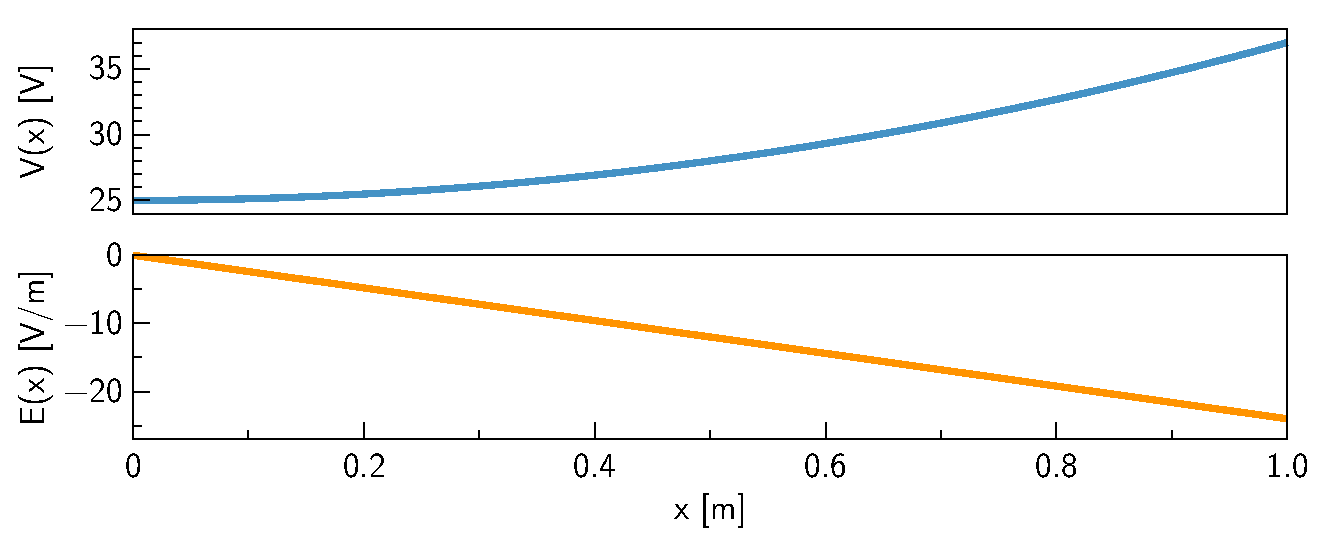
\includegraphics[width=0.7\textwidth]{figs/pot1d.pdf}
\end{center}

\end{frame}

\begin{frame}
\frametitle{Lorentz force and magnetic field}
\small
The Lorentz force depends on both the magnetic field $\vc{B}$ and the velocity $v$ of a charge $q$
\begin{equation}
	\vc{F}_m=q \vc{v} \times \vc{B},
\end{equation}
It is perpendicular to both $\vc{v}$ and $\vc{B}$ and the $\vc{v}$ dependence makes it \textbf{non-conservative}.\newline

%Important: the force is caused by the particle motion, not vice-versa.\newline

The work performed by $\vc{F}_m$  along any path is identically \textbf{zero}

\begin{equation}
	\int_i^f \vc{F}_m\cdot d\vc{\ell}=q\int_i^f  (\vc{v} \times \vc{B})\cdot d\vc{v}dt=0,
\end{equation}
(the scalar product of orthogonal vectors is zero).\newline
%
%\hl{The magnetic field does \textbf{no work} on the point charge}. We can formally define a potential $V_B$ such that $-\text{grad}V_B = \vc{B}$, but we cannot link it -in general- to a physical force.
\end{frame}

\begin{frame}
	\frametitle{Magnetic vs electric field}

	For the electric field, we can write the force on a point charge as $\vc{F}_e = q\vc{E}$.\newline
	
	For the magnetic field $\vc{B}$, the force is not simply proportional to the field, and there are \textbf{no magnetic charges}. 
	
	The construction of the scalar potential $V$ from $\vc{E}$ \textbf{cannot be repeated }for $\vc{B}$.\newline
	
	\end{frame}

\begin{frame}
\frametitle{Magnetic vs electric field}

	In fact, the difference between $\vc{E}$ and $\vc{B}$ can be mathematically cast in terms of \textbf{circulation}
	\begin{align}
		\oint_C \vc{E}\cdot d \vc{\ell}&=0\\
		\oint_C \vc{B}\cdot d \vc{\ell}&=\mu_0 I_C\neq0\\
	\end{align}
	where $I_C$ is the current through the closed loop $C$. \newline More on this in the next sessions.\newline
	
	
\end{frame}




\begin{frame}
\frametitle{Take-home messages}
\begin{enumerate}
	\item For conservative forces, the work done between two points in space is path-independent.
	\item The electrostatic field $\vc{E}$ is a \textbf{conservative vector field} with potential $V$:
	\begin{itemize}
	\item integral form $V_f-V_i=-\int_i^f \vc{E} \cdot d\vc{\ell}$
	\item local form $-\text{grad} V = \vc{E}$
	\end{itemize}
	\item There is no scalar potential for the magnetic field $\vc{B}$.
\end{enumerate}

\textbf{Remember:} al this is valid for \textbf{static} (= time independent) electric (and magnetic) fields.
\end{frame}

\end{document}